%% 
%% Copyright 2007-2020 Elsevier Ltd
%% 
%% This file is part of the 'Elsarticle Bundle'.
%% ---------------------------------------------
%% 
%% It may be distributed under the conditions of the LaTeX Project Public
%% License, either version 1.2 of this license or (at your option) any
%% later version.  The latest version of this license is in
%%    http://www.latex-project.org/lppl.txt
%% and version 1.2 or later is part of all distributions of LaTeX
%% version 1999/12/01 or later.
%% 
%% The list of all files belonging to the 'Elsarticle Bundle' is
%% given in the file `manifest.txt'.
%% 
%% Template article for Elsevier's document class `elsarticle'
%% with harvard style bibliographic references

\documentclass[preprint,12pt,authoryear]{elsarticle}
\usepackage[margin=2.5cm]{geometry} % uniform 2.5 cm margin
%% Use the option review to obtain double line spacing
%% \documentclass[authoryear,preprint,review,12pt]{elsarticle}

%% Use the options 1p,twocolumn; 3p; 3p,twocolumn; 5p; or 5p,twocolumn
%% for a journal layout:
%% \documentclass[final,1p,times,authoryear]{elsarticle}
%% \documentclass[final,1p,times,twocolumn,authoryear]{elsarticle}
%% \documentclass[final,3p,times,authoryear]{elsarticle}
%% \documentclass[final,3p,times,twocolumn,authoryear]{elsarticle}
%% \documentclass[final,5p,times,authoryear]{elsarticle}
%% \documentclass[final,5p,times,twocolumn,authoryear]{elsarticle}

%% For including figures, graphicx.sty has been loaded in
%% elsarticle.cls. If you prefer to use the old commands
%% please give \usepackage{epsfig}

%% The amssymb package provides various useful mathematical symbols
\usepackage{amssymb}
%% Useful packages
\usepackage{tabularx}
\usepackage{amsmath}
\usepackage{graphicx}
\usepackage[colorlinks=true, allcolors=blue]{hyperref}
\usepackage{caption}
\usepackage{subcaption}
\usepackage{sectsty}
\usepackage{float}
\usepackage{subfiles}
\usepackage{soul}

%% The amsthm package provides extended theorem environments
%% \usepackage{amsthm}

%% The lineno packages adds line numbers. Start line numbering with
%% \begin{linenumbers}, end it with \end{linenumbers}. Or switch it on
%% for the whole article with \linenumbers.
%% \usepackage{lineno}

\journal{The Journal of Transport Geography}

\begin{document}

\begin{frontmatter}

%% Title, authors and addresses

%% use the tnoteref command within \title for footnotes;
%% use the tnotetext command for theassociated footnote;
%% use the fnref command within \author or \affiliation for footnotes;
%% use the fntext command for theassociated footnote;
%% use the corref command within \author for corresponding author footnotes;
%% use the cortext command for theassociated footnote;
%% use the ead command for the email address,
%% and the form \ead[url] for the home page:
%% \title{Title\tnoteref{label1}}
%% \tnotetext[label1]{}
%% \author{Name\corref{cor1}\fnref{label2}}
%% \ead{email address}
%% \ead[url]{home page}
%% \fntext[label2]{}
%% \cortext[cor1]{}
%% \affiliation{organization={},
%%            addressline={}, 
%%            city={},
%%            postcode={}, 
%%            state={},
%%            country={}}
%% \fntext[label3]{}

\title{How Demand Responsive Transport Systems Can Protect Cape Town's Overburdened Traffic Systems from Congestion Collapse}

%\title{Simulating Demand Responsive Transport for Urban Congestion Mitigation: A Cape Town Case Study with Global South Implications}

%% use optional labels to link authors explicitly to addresses:
%% \author[label1,label2]{}
%% \affiliation[label1]{organization={},
%%             addressline={},
%%             city={},
%%             postcode={},
%%             state={},
%%             country={}}
%%
%% \affiliation[label2]{organization={},
%%             addressline={},
%%             city={},
%%             postcode={},
%%             state={},
%%             country={}}

\author[inst1]{Alexander Röhrs}

\affiliation[inst1]{organization={Chair of Data Science, Faculty of Management, Construction and Real Estate, HAWK},Department and Organization
            addressline={Haarmannplatz 3}, 
            city={Holzminden},
            postcode={37603}, 
            state={Lower Saxony},
            country={Germany}}

\author[inst2]{Estelle Stambolie}
\author[inst1]{Andreas Bossert}
\author[inst3]{Obiora Nnene}
\author[inst3]{Mark Zuidgeest}
\author[inst1,inst2]{Jan Chr. Schlüter}

\affiliation[inst2]{organization={Department of Economics, University of Göttingen},Department and Organization
            addressline={Humboldtallee 3, 37073 Göttingen, Germany}, 
            city={Göttingen},
            postcode={37073}, 
            state={Lower Saxony},
            country={Germany}}

            \affiliation[inst3]{organization={Centre for Transport Studies, Department of Civil Engineering, University of Cape Town},Department and Organization
           addressline={Rondebosch}, 
            city={Cape Town},
           postcode={7701}, 
           state={Western Cape},
           country={South Africa}}





\newpage
\begin{abstract}
%% Text of abstract

%By employing relative fleet sizing and pricing schemes this study establishes a scalable baseline that is independent of site-specific absolute values, facilitating direct transferability to other regions worldwide

%A key trade-off is that while average car travel times decreased by 12-17 minutes, public transport trip times increased in service areas, highlighting the need for operational optimization. 

Cape Town, South Africa, is a highly congested city requiring urgent intervention to curb private motorized transport. Existing minibus taxis as well as non-shared ride-hailing services like Uber and Bolt have failed to alleviate, and arguably exacerbated, this problem. Demand-responsive transport (DRT) emerges as a promising sustainable alternative. While the potential risks, like public transport cannibalization, are widely debated, their practical implications in the context of the Global South are under-researched. To address this gap, we simulate the operation of a hypothetical large-scale shareable DRT service in Cape Town using an Agent-Based Transport Simulation (MATSim). By employing relative fleet sizing and pricing schemes this study establishes a scalable baseline that is independent of site-specific absolute values, facilitating direct transferability to other regions worldwide. Our findings show that DRT can reduce citywide congestion by up to 28.2\,\% (up to 50\,\% in buffer areas), demonstrating its potential to alleviate traffic bottlenecks. Critically, it facilitated multi-modal trips, increasing overall public transport usage without significant cannibalization. Effectiveness was maximized by competitive pricing and larger fleets, with shared rides (between 25\,\% and 40\,\% of DRT trips) mitigating dead mileage. While our simulation results demonstrate substantial congestion relief under the assumption of rational mode-choice responses, real-world adoption in Cape Town may be moderated by socio-behavioural barriers. Persistent distrust in shared systems, heightened concerns over personal safety, and the entrenched social status of private car ownership often lead commuters to prefer private vehicles even under severe congestion. Acknowledging these factors, this study nonetheless provides policy-relevant recommendations for the Global South cities in general, Cape Town in particular, and offers a transferable methodological framework for other congested metropolises worldwide.

\end{abstract}


%%Research highlights
\begin{highlights}
\item DRT reduced citywide congestion by up to 28.2\%, with buffer areas experiencing reductions of up to 50\%, demonstrating its potential to alleviate urban traffic bottlenecks.
\item DRT facilitates multi-modal trips, increasing public transport usage without significant cannibalization, supporting sustainable urban mobility in Cape Town.
\item Average car travel trip times decreased by 12--17 minutes, but public transport trips in service areas saw increases, highlighting the need for operational optimization.
\item Competitive pricing and larger fleets maximize DRT’s effectiveness, with shared rides (25--40\% of trips) offsetting dead mileage caused by re-allocation of empty DRT vehicles.
\item The study analyzes the spatial distribution of congestion changes following DRT introduction, revealing pronounced relief in the CBD and buffer zones while highlighting varying impacts across service areas.
\end{highlights}

\begin{keyword}
%% keywords here, in the form: keyword \sep keyword
Demand Responsive Transport \sep Transport Systems \sep Congestion \sep Overburdened Traffic Systems \sep MATsim \sep Cape Town \sep South Africa
%% PACS codes here, in the form: \PACS code \sep code
%\PACS 0000 \sep 1111
%% MSC codes here, in the form: \MSC code \sep code
%% or \MSC[2008] code \sep code (2000 is the default)
%\MSC 0000 \sep 1111
\end{keyword}

\end{frontmatter}

%% \linenumbers

%% main text
\newpage

\subfile{introduction}

\subfile{literature}

\subfile{method}

\subfile{results_new}

\subfile{discussion}


%\subfile{conclusion}
%\begin{figure}[h]
%\centering
%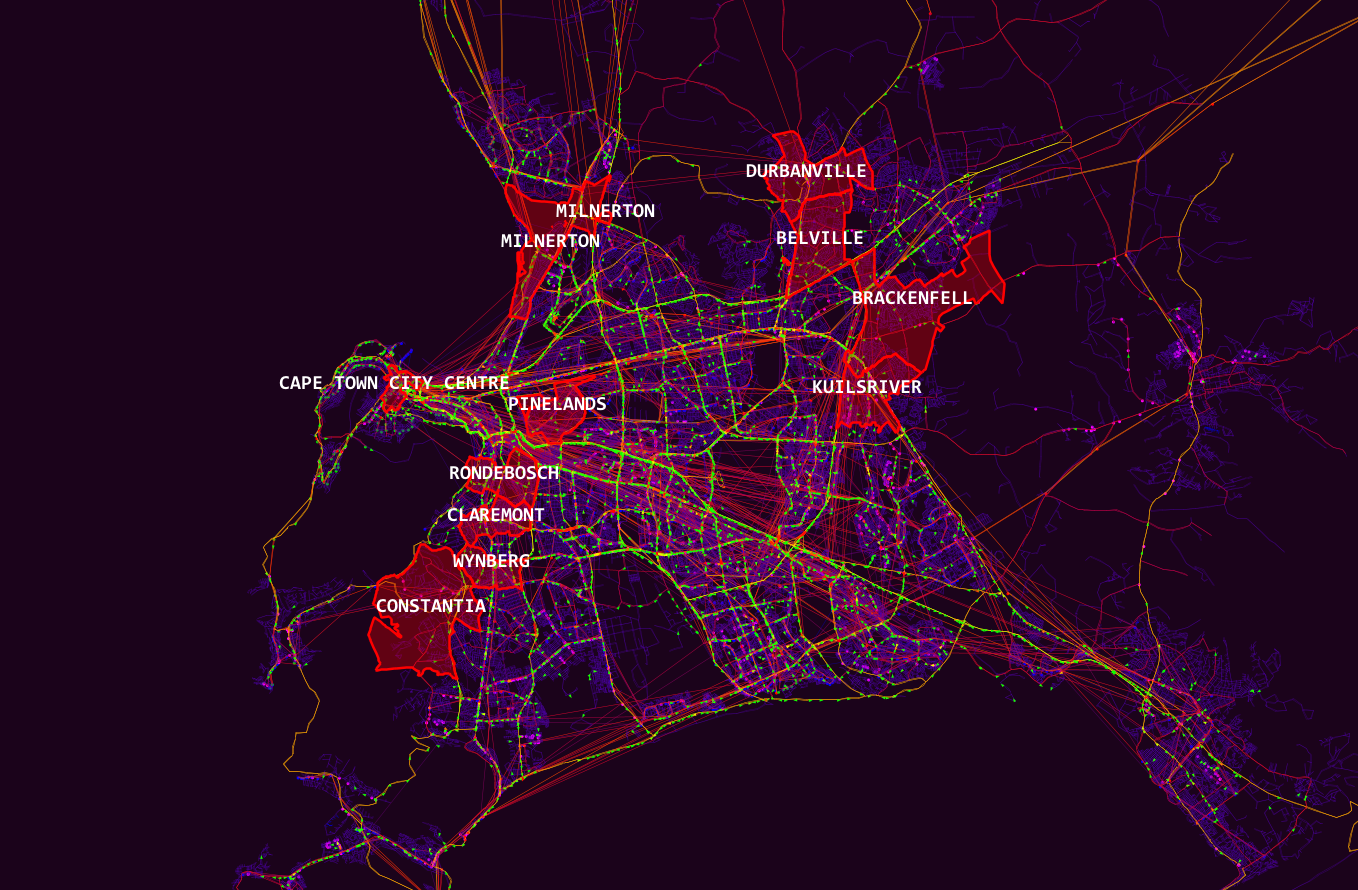
\includegraphics[width=.9\textwidth]{images/drt_service_areas_via.png}
%  \captionsetup{width=.9\textwidth}
%  \caption{Visualization of MATSim Simulation with DRT Service Areas in Capetown (red-%filled polygons).}
 % \label{fig:7}
%\end{figure}



\newpage
%% If you have bibdatabase file and want bibtex to generate the
%% bibitems, please use
%%
%\bibliographystyle{elsarticle-harv} 
\bibliographystyle{elsarticle-harv} 

\bibliography{my_ref}
%% If you have bibdatabase file and want bibtex to generate the
%% bibitems, please use
%%
%\bibliographystyle{elsarticle-harv} 
%\bibliography{ref}

%% else use the following coding to input the bibitems directly in the
%% TeX file.

% \begin{thebibliography}{00}

% %% \bibitem[Author(year)]{label}
% %% Text of bibliographic item

% \bibitem[ ()]{}

% \end{thebibliography}
\newpage
\appendix

%\subfile{appendix}

\end{document}

\endinput
%%
%% End of file `elsarticle-template-harv.tex'.